Image reconstruction is necessary to produce images of activity distribution from the acquired tomographic measurements. Reconstruction algorithms used for this process can be categorised as either analytical or statistical reconstruction methods.  
Analytical reconstruction methods seek to invert the transformation that links the image to the data domain, using linear analytic approaches. These methods treat the measured LOR data as line integrals over image space and necessitate corrections to be applied on projection data prior to reconstruction, in order to result in valid and quantitatively accurate images. Traditionally the most commonly used analytical reconstruction method is \textit{Filtered Back Projection} which is described very briefly in this chapter. 
Statistical reconstruction methods are derived from statistical formulations of the detection process and allow for the use of complex system models that include various effects of the acquisition process. These methods result in non-linear formulations of the reconstruction problem which require iterative optimisation methods to reach a solution. The solution sought is a set of image parameters (that describe the activity distribution) that best describes the acquired tomographic data. 
In this thesis project, we made exclusive use of statistical reconstruction methods due to their ability to incorporate complex system models, including the use of dynamic models which was crucial for the aims of this thesis.

\section{Projection and back-projection process}
Coincidence detection of annihilation photons in PET leads naturally to a line-integral model where the number of coincidence events of an \gls{lor} is approximately linearly proportional to the integral of tracer density along the volume joining the two detectors. 
The projection process can be written as
\begin{equation}
   \bm y = proj\{\bm{\lambda}\}  \\, 
  \label{eqn:Radon}
\end{equation}
where $\bm{\lambda}$ is the continuous distribution of radiotracer and $\bm{y}$ the continuous projection data (or else sinogram data).
The 2D projection operation is also known as the Radon transform~\cite{radon1917,Radon1986} and translates from the image to the projection data domain. Projections in 3D can be made using the X-ray transform or extension of the Radon transform~\cite{Natterer1986}. 
The projection's dual operation is back-projection, which translates from the data domain to the image domain.
%
\subsection{Image representation}
In practice, the spatio-temporal radiotracer distribution is described using a model with a finite number of parameters. The most common choice in common practice is the use of equally sized non-overlapping voxels that cover the useful \gls{fov}. Their use can also extend to the temporal domain with a set of voxels describing the \gls{fov} for each temporal bin. In this case, the sets of voxels per temporal bin are considered temporally independent.
If for a moment we consider only the spatial domain and static imaging, we can model the spatial radiotracer distribution $\bm{\lambda}$ using voxels with the  $rect$ function as
\begin{equation}
   g(\bm{r};\bm\lambda) = \sum_{j=1}^{n_{j}} \lambda_j {rect}(\bm{r}-\bm{r}_j)  \\, 
\end{equation}
for an ${n_{j}}$ number of voxels with $r_j$ coordinates and intensity $\lambda_j$.
For the linear model case, the set of functions describing the distribution are referred to as \textit{spatial basis functions}. From here on we will be using the $\bm\lambda$ symbol to refer to the ${n_{j}}$ dimension vector of $\lambda_j$ voxel weights that describe the spatial activity distribution as 
\begin{equation}
   \bm\lambda = \big\{ \lambda_j| j=1,\cdots,n_j \big\} \\.
\end{equation}
If we now consider the temporal domain of the activity distribution as well, the $rect$ function can be used 
on the time domain to define a set of $n_t$ independent temporal bins (frames). Later in this chapter, we will show how dynamic models can be used to describe the behaviour of voxel values across the temporal domain, but traditional reconstruction treats frames as independent static detests.
In this case, the activity distribution of each frame can be written as
%\begin{equation}
%   \bm{\lambda} = \Big\{ {\bm{\lambda}_m,m=1,..,n_m} \Big\} \\,
%\end{equation}
%where
\begin{equation}
   \bm{\lambda_t} = \big\{ {\lambda_{tj}| j=1,\cdots,n_j} \big\} \\.
\end{equation}
Equivalently the projection data are binned according to the discretization imposed by the \glspl{lor} in $y_i$, where $i$ is the projection bin index and $n_i$ the total number of \glspl{lor}. Similarly to the image data, the projection data are binned temporally into $y_{ti}$ for each projection bin $i$ at frame $t$ for a total number of number of $n_t$ frames. 
The data of each frame can then be written as
%\begin{equation}
%   \bm{y} = \Big\{ {\bm{y}_m,m=1,...,n_m} \Big\} \\,
%\end{equation}
%where
\begin{equation}
   \bm{y_t} = \big\{ {y_{ti}| i=1,\cdots,n_i} \big\} \\.
\end{equation}
%
\subsection{Projection \& Analytical reconstruction}
Forward projection of image to data space can be treated by summing contributions of voxels across each~\gls{lor}. %Different projection strategies exist that model the contribution of voxels differently depending on their placement in the \gls{lor}. 
As this is a computationally heavy process in practice, different methods have been proposed that balance between accuracy and consistency and computing requirements. %A short follows list with basic description of the methods that are implemented in CASToR.
Some of these methods, which are also implemented in the CASToR reconstruction software, are listed below with a short description.
\begin{itemize}
\item  \textbf{Siddon projector}~\cite{Siddon1985}: Weights the contribution of an LOR to each by the length of the line that intersects the voxel.
\item  \textbf{Distance driven}~\cite{DeMan2004}: An optimised method for calculating weights by mapping pixel boundaries and detector boundaries for each projection to a common axis .
%\item  \textbf{Incremental Siddon}~\cite{Jacobs2015}:
\item  \textbf{Joseph}~\cite{Joseph1982}: Estimates contribution of voxels to LOR based on linear interpolation and their distance from the LOR. 
\item  \textbf{Multi-Siddon}~\cite{Moehrs2008}: Uses multiple lines from the faces of the detectors in each LOR to approximate the volume intersected between the two detectors and the voxel.
\end{itemize}

%\begin{figure} [h!]
%\centering
%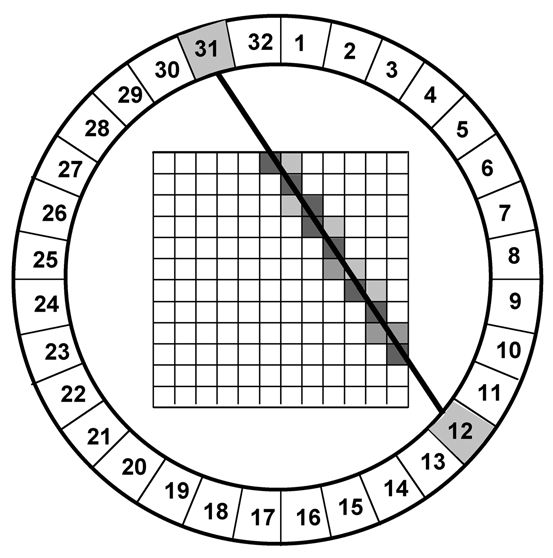
\includegraphics[scale=0.35,angle=0]{2_Theory_Methods/figures/Radon_Discrete.png}
%\caption{Back-projection of a single LOR through image space, with contribution weighted according to the length of the line that intersects the voxel.} 
%\label{fig_3:back_projection.}
%\end{figure} 
Similarly, the back-projection operation assigns to voxels in the \gls{fov} the contribution from each \gls{lor} bin, using the same methods.
Analytical reconstruction methods seek to estimate an image by inversion of the forward-projection process, by superimposing contributions from all \glspl{lor} in image space. 
This results in analytical algorithms, including the most widely used algorithm of \textit{Filtered Back Projection} (FBP).
%In practice a filtered version of the projections is back-projected to account for the non-uniform number of contributions from LORs in different regions of the image space, which gives the processes the name of filtered back projection. The method can be extended to 3D via use of the 3D X-ray transform and approximations of missing data projections~\cite{Kinahan1989}. 
But while analytical reconstructions are linear processes and computationally fast, accuracy is limited by the simplistic assumptions of the line integral model, ignoring many degrading effects such as positron range, variations in response across \glspl{lor} etc. In addition, these methods do not account for the statistical properties of the detection process in the data.
Finally, the FBP algorithm seeks to solve an ill-posed problem meaning that small changes in the data can result in largely disproportional effects on the reconstructed image. As the projection data include stochastic noise from the detection process, the reconstruction suffers from artefacts. In practice, smooth low pass filters like the Hann apodization filter are applied in the reconstruction process to reduce the strength of these artefacts at the cost of degraded spatial resolution. The sub-optimal trade-off between strength of artefacts and spatial resolution can be adjusted by changing the filter's cut-off frequency.

\section{Formulation of the system model}
The analytical reconstruction methods are based on the idealised description of the scanning process using the line integral model. But in fact, there are many effects that should ideally be considered in the scanning system model. For example the statistical nature of the detection process, positron range and detection resolution effects, the detection of scattered and random events as well as the discrete nature of the detection and scanner geometries that do not result in complete sampling.
But as the scanning model complexity is increased, analytic expressions that seek to inverse the scanning process are not feasible.
For this reason, iterative algorithms are employed, which seek a solution by optimising an objective function that expresses some difference measure between the measured data and the modelled data from an image estimate.

We can define the system model using an $n_i \times n_j$ system matrix $\bm{P}$. Each element $P_{ij}$ of the matrix is the probability of detection by voxel $j$ to data bin $i$. 
As discussed, many effects can be included in this matrix elements which will be outlined below. By contrast, scatter effects can be hard to implement in the system matrix and random effects are non-linear effects that cannot be modelled linearly. As such the scatter and random events are considered to be known for each detector bin and included as an additive background $b_i$ for each data bin $i$ in the system model.

The model of the data at bin $i$ from an image $\bm{\lambda}$ can be written as a sum over voxels of the probability of detection in this bin 
\begin{equation}
   \hat{y_i} = \sum_{j=1}^{n_j} P_{ij} \lambda_j + b_i ,
   \label{eqn:system_model}
\end{equation}
where $\hat{y_i}$ is the modelled data or expectation of the data.

The system matrix can be decomposed to the individual contributing components as separate sparse matrices and vectors
\begin{equation}
   \hat{y_i} = n_i a_i \sum_{j=1}^{n_j} X_{ij} \sum_{k=1}^{n_j} H_{jk} \lambda_{jk} + b_i ,
\end{equation}

where
\begin{itemize}
    \item $n_i$ are the normalisation factors for each LOR bin
    \item $a_i$ are the attenuation factors for each LOR bin
    \item $X_{ij}$ is the geometrical projection matrix
    \item $H_{jk}$ is the resolution modelling matrix, applied as a convolution in image space
    \item $b_i$ the background events for each LOR bin.
\end{itemize}
%
Resolution modelling can be applied on both data and image space of the system model, but in practice is applied on one of the two domains~\cite{Stute2013}. In the CASToR reconstruction software that was used in this project, resolution modelling is implemented in image space as written in the above expression.

If \gls{tof} measurements are available, the additional information regarding the probability of the annihilation event along the \gls{lor} can be incorporated in the model. \Gls{tof} weights are assumed to be independent of the other system matrix elements and thus act as an additional multiplication factor. Depending on the type of \gls{tof} information, the weights can either be quantized (for each \gls{tof} bin) or expressed as a continuous function. More details on both options and the implementation of \gls{tof} reconstruction can be found in the work of Filipović~\textit{et al.}~\cite{Filipovic_2019}. 
%
\section{Formulation of the objective function}
%As discussed above, iterative reconstruction relies in optimisation of an objective function. 
We can consider the total number of events in each projection bin to be modelled as a random sample from a Poisson distribution. According to the probability mass function, the conditional probability or likelihood function for $\hat{y_i}$ given the measured data ${y_i}$ will be
\begin{equation}
p({y_i}|{\hat{y_i}}) = L({\hat{y_i}}|{y_i}) = e^{-\hat{y_i}} \frac{\hat{y_i}^{y_i}}{{y_i}!}  \\  .
\end{equation}
With the assumption that measurements of counts in each bin are independent random processes, the likelihood of the data over all bins will be
\begin{equation}
p(\bm{y}|\bm{\hat{y}}) = L(\bm{\hat{y}}|\bm{y}) = \prod_i^{n_i} e^{-\hat{y_i}} \frac{\hat{y_i}^{y_i}}{{y_i}!} . 
\label{eqn:probability}
\end{equation}
By substituting the system model equation \ref{eqn:system_model} in equation~\ref{eqn:probability}, we can write an expression of likelihood of the image $\bm{\lambda}$ given the measured data $\bm{y}$.
\begin{equation}
    L(\bm{\lambda}|\bm{y})  = \prod_i^{n_i} e^{-(\sum_{j=1}^{n_j} P_{ij} \lambda_j + b_{i} )} \frac{(\sum_{j=1}^{n_j} P_{ij} \lambda_j + b_{i} )^{y_i}}{{y_i}!}
\end{equation}
This expression can be used as the objective function in the optimisation process of seeking the most likely (ML) estimate of $\bm{\lambda}$ from a measurement $\bm{y}$ . 
It is more convenient to take the expression of the log likelihood and since the log function is monotonic the log likelihood can be used to arrive to the same ML estimate.

The log likelihood expression is
\begin{equation}
    lnL(\bm{\lambda}|\bm{y})  = \sum_{i=1}^{n_i}\left[ y_i ln(\sum_{j=1}^{n_j} P_{ij} \lambda_j + b_i) -\sum_{j=1}^{n_j} P_{ij} \lambda_j - b_i - ln({y_i}!) \right] \\.
\label{eqn:log_likelihood}
\end{equation}
This expression of the Poisson log-likelihood will be used to arrive to the maximum likelihood estimate image $\bm\lambda$, which will be noted as $\bm{\lambda}^{ML}$, that maximises the likelihood of the modelled data given the measured \mbox{data $\bm{y}$}. 
\begin{equation}
\bm{\lambda}^{\textrm{ML}} = \argmax{\bm{\lambda}}(lnL(\bm{\lambda}|\bm{y}))
\end{equation}
\section{Maximum Likelihood - Expectation Maximisation}
\label{section:MLEM}
The second partial derivative of the log-likelihood to $\lambda_j$ can be shown to be negative semidefinite to all allowed images and thus the log-likelihood function is a concave function. This means that a found local maximum through the optimisation process will be the global maximum of the function.

Seeking to solve equation~\ref{eqn:log_likelihood} to find analytically the maximum likelihood image $\bm{\lambda}^{ML}$, we can take its first partial derivative to $\lambda_j$ and set it to be equal to zero. 
\begin{equation}
\frac{\partial lnL(\bm{\lambda}|\bm{y})}{\partial \lambda_j} = \sum_{i=1}^{n_i}\left[  y_i \frac{\sum_{j=1}^{n_j} P_{ij} }{\sum_{j=1}^{n_j} P_{ij} \lambda_j + b_i} -\sum_{j=1}^{n_j} P_{ij}
\right]  = 0 \\,
\end{equation}
but this expression has no closed form solution.
The arrival to this expression shows the need for iterative methods to seek the $\bm{\lambda}^{\textrm{ML}}$ solution. 

The most common algorithm used for this problem is the Expectation Maximisation algorithm that was first applied on statistical PET reconstruction by two key works by Shepp and Vardi~\cite{Vardi1985} and Lange and Carson~\cite{Lange1984}. In these works the solution is derived through the introduction of the "complete data" concept~\cite{Dempster1977}. \\
Let $\bm{z}$ be the complete data random dataset of $x_{ij} + g_i$ values which describes the exact number of emissions from voxel $j$ that contribute to the measurement at projection bin $i$, with the many to one mapping 
\mbox{$y_i = \sum_{j=1}^{n_j} x_{ij} + g_i$}.
The complete dataset is unknown, but the conditional expectation of the complete data can be expressed using an image estimate (a guess) noted as $\bm{\lambda}^{(k)}$ and the measured data $\bm{y}$ as 
%
\begin{equation}
\label{eq:Complete_Data_Expectation1}
\hat{x}_{ij}(\bm{\lambda}^{(k)},y_i) = y_i
\frac{P_{ij} \lambda_j^{(k)}}{\sum_{d=1}^{n_j} P_{id}\lambda_d^{(k)} + b_i} \\ , 
\end{equation}
%
\begin{equation}
\label{eq:Complete_Data_Expectation2}
\hat{g}_{i}(\bm{\lambda}^{(k)},y_i) = y_i 
\frac{b_i}{\sum_{d=1}^{n_j} P_{id}\lambda_d^{(k)} + b_i} . 
\end{equation}
%

The complete dataset follows a Poisson distribution, with its log-likelihood being
\begin{equation}
lnL(\bm{\lambda}|\bm{z}) = 
\sum_{i=1}^{n_i} \left[\sum_{j=1}^{n_j}( x_{ij} ln(P_{ij}\lambda_j) - P_{ij} \lambda_j) +
g_i ln(b_i) - b_i \right] \\ ,  
\label{eqn:log_likelihood_z}
\end{equation}
where parameters not related to its optimisation to $\lambda$ have been dropped. 
If we replace the expectation of the complete data using equations~\ref{eq:Complete_Data_Expectation1} and ~\ref{eq:Complete_Data_Expectation2} we can then seek to maximise this likelihood function to obtain the ML image estimate of the expected complete data. Using the Kuhn-Tucker conditions we arrive at a closed form solution
\begin{equation}
\lambda_j^{(k+1)} = \frac{\lambda_j^{(k)}}{\sum_{i=1}^{n_i} P_{ij}} 
\sum_{i=1}^{n_i} P_{ij} 
\frac{y_i}{\sum_{d=1}^{n_j} P_{id}\lambda_d^{(k)} + b_i } \\,
\label{eqn:MLEM}
\end{equation} 
that provides a new estimate $\bm{\lambda}^{(k+1)}$. This single update equation combines the two steps of the optimisation process. First, given an image estimate $\bm{\lambda}^{(k)}$ the expectation of the complete data is estimated. Then, the log-likelihood of the expectation of the complete data is maximised. This iterative process results in monotonic increase of the original log-likelihood function. This process is the \textit{MLEM} algorithm.
%Together with the expression for the conditional expectation of the complete data, the two step process of Expectation Maximisation and  Maximum likelihood estimation can be written in a single update equation. Given data $\bm{y}$ and an image estimate $\bm{\lambda}^{(k)}$ , the updated image estimate $\bm{\lambda}^{(k+1)}$ is given from:
%This equation forms a single update of the MLEM algorithm, which when evaluated over all voxels $j$ provides an updated image $\bm{\lambda}^{(k+1)}$. 

The use of the conditional expectation of the data is an example of the general concept of optimisation transfer, where the construction of surrogate functions is made to be used with a simpler optimisation process, that leads to optimisation of the main function as well. One advantage of this algorithm is that an update over all voxels of the image can be made with a single pass over the data. The disadvantage is that it results in very slow convergence speeds. 
To accelerate convergence the Ordered Subsets algorithm is used in most practices, which makes use of subsets of the data at each update step (each subset) to reduce computing time for each image update. 

\section{Dynamic reconstruction}
\label{section:Fully_4D_reconstruction}
Soon after the proposition of the EM algorithm for iterative PET reconstruction by Shepp and Vardi~\cite{Vardi1985} and Lange and Carson~\cite{Lange1984}, the former group proposed an extension of the EM algorithm to update parameters of a dynamic model and a version of the update algorithm that iterates through the whole of dynamic PET data in each iteration~\cite{Carson1985}. Dynamic PET data are traditionally divided among many time bins (frames) resulting in limited counts in each frame. Independent reconstruction of each frame dataset and post-reconstruction kinetic modelling results in noisy and potentially biased parameter estimates. Furthermore, the noise in each frame image estimate is spatially correlated and is hard to be accounted for in the post-reconstruction modelling. The use of a dynamic reconstruction approach that updates over parameters using all the dynamic PET raw data offers the advantages of accurate noise modelling of the raw data and accurate system modelling directly in the process of the dynamic model parameter estimation. Unfortunately, one major disadvantage of this approach was very slow convergence properties making it difficult for use in practice and the topic was not researched further at that time~\cite{Carson1985}. \\
More than 10 years later the approach was revisited by Matthews \textit{et al}~\cite{Matthews1995} where it was combined with linear models. As it will be shown in this chapter the MLEM algorithm can be easily extended to parametric space with the use of linear dynamic models. On their application, the benefits in reducing parametric image noise were seen, at the cost of very slow convergence speeds. For use with linear models, attempts to accelerate convergence were made by use of OSEM~\cite{Tsoumpas2008} and computing acceleration and compression techniques~\cite{Hong2008}. In the case of dynamic reconstruction with OSEM it was shown that the algorithms exhibits the common OSEM problem of limit-cycles, for which a decreasing subsets scheme was used to eliminate this effect~\cite{Angelis2011}. \\
It was not until the work of two groups in 2010, Wang \textit{et al}~\cite{Wang2010} and Matthews \textit{et al}~\cite{Matthews2010}, that allowed for practical and more widespread use of dynamic reconstruction. Their methods, based on principles of optimisation transfer by Lange~\cite{Lange2000}, decouple the dynamic reconstruction process to an EM update over all data and to an ML problem in image space. The first step iterates through the tomographic data and updates the activity estimate images, while the second simply updates the dynamic model parameters using the updated activity images. With the second step being much faster, multiple dynamic model updates can be conducted for each update over data which results in acceleration of overall convergence. Results were demonstrated by Wang \textit{et al}~\cite{Wang2010} for EM and PCG based optimisations using linear models. While that work was limited to linear dynamic models, the work by Matthews \textit{et al}~\cite{Matthews2010} generalised on the optimisation of the image space ML problem by the use of an equivalence to a weighted least-square minimisation problem. This formulation allowed for use of existing LS optimisation algorithms, that are commonly used for post-reconstruction model fitting, to be used in 4D reconstruction for linear and non-linear models. The disadvantage of this approach is that the resulting formulation is not strictly concave and thus does not guarantee monotonic convergence to a global maximum. Nevertheless, convergence behaviour has been observed in practice with different weighting schemes~\cite{Gravel2015,Wang2013}. \\
The use of non-linear models within dynamic reconstruction has shown clear benefits in precision and accuracy~\cite{Angelis2014,Kotasidis2012,Gravel2015} but are more sensitive to initialisation and reconstruction parameters and could lead to unpredictable behaviour.

\subsection{Dynamic models}
As described in chapter~\ref{Chap2_2:Pharmacokinetics}, dynamic data are used to seek parameters of kinetic models for the understanding of underlying molecular processes. Conventionally the data of each frame are reconstructed individually as individual static datasets and the result images are used for post-reconstruction modelling. When the parameters sought are calculated at the voxel level, the result is a set of parameters for each voxel in the FOV, which are referred to as parametric maps.


If we assume an example dynamic model that describes the dynamic behaviour of the radiotracer distribution with $n_p$ number of $p$ parameters, then the set of parameters for each voxel $j$ can be expressed as
\begin{equation}
   \bm{\theta_j} = \big\{ {\theta_{pj}| p=1,\cdots,n_p} \big\} \\.
\end{equation}
These can be used to model the activity behaviour at each time frane $t$ according to
\begin{equation}
   \lambda_{tj} = f_{tj}(\bm\theta_{j}) \\,
\label{eqn:LinearDynamicModel}
\end{equation}
where $f()$ is the function of the dynamic model that estimates radiotracer activity values over $n_t$ time frames given a set of $n_{p}$ model parameters.
Assuming that the dynamic model is the same for all voxels in the image space, we can write for short 
\begin{equation}
\bm\lambda = f(\bm\theta) \\, 
\end{equation}
with the complete set of parametric maps and spatio-temporal images being respectively
\begin{equation}
   \bm{\theta} = \big\{ {{\theta}_{pj}|p=1,\cdots,n_p ; j=1,\cdots,n_j} \big\} , 
\end{equation}
\begin{equation}
   \bm{\lambda} = \big\{ {{\lambda}_{tj}|t=1,\cdots,n_t ; j=1,\cdots,n_j} \big\} \\. 
\end{equation}
The dynamic model $f()$ can be either linear or non-linear to the set of parameters $p$. 
%When the spatio-temporal data $\bm{\lambda}$ are reconstructed form individual 3D frame reconstructions they commonly result in high noise in the activity distribution images due to the limited counts in each time frame. When  the dynamic model parameters are sought or parametric images, the dynamic or kinetic model is fitted post-reconstruction. Especially in the case of parametric images the noise of the individual 3D frame data results in noisy and potentially biased parametric images. This two step process not only results in noise parametric images but also does not account for the noise in the PET data in the post-reconstruction fitting process.
%Instead of this two-step process, it is possible to derive reconstruction algorithms that include dynamic models and can be applied on the whole of the dynamic PET data. These reconstruction algorithms, which are referred to as 4D reconstruction algorithms due to their application in 4 dimensions, seek to reduce the problem of limited counts that would else be used in individual frame bins by making use of the whole of the dynamic PET data. The dynamic models used are chosen to provide meaningful constrains and when the model of interest that would otherwise be used post-reconstruction is included, the 4D reconstruction algorithms can directly provide the parameters and parametric images of interest.
%Typically (although its not always the case) the number of parameters of dynamic models is smaller than the number of time frames in a study and so the use of 4D reconstruction effectively reduces the number of parameters to estimate, that along with the constraints imposed by the dynamic model result in an important reduction of noise and potentially improved bias. Furthermore direct use of dynamic models in reconstructions allows for the use of the noise-model that describes the PET data detection to be accounted for in the estimation of the final dynamic model parameters.
\subsection{Dynamic reconstruction - Nested optimisation}
Similar to~\ref{section:MLEM}, the conditional expectation of the complete data can be written using the generic dynamic model $f()$  
\begin{equation}
\label{eq:Dynamic_complete_Data_Expectation}
\hat{x}_{tij}(\bm{\theta}^{(k)},y_{ti}) = y_{ti}
\frac{P_{ij} f_{tj}(\bm\theta^{(k)})}
{\sum_{d=1}^{n_j} P_{id} f_{td}(\bm\theta^{(k)}) + C_{ti}}\\,
\end{equation}
%
\begin{equation}
\label{eq:Dynamic_complete_Data_Expectation2}
\hat{g}_{ti}(\bm{\theta}^{(k)},y_{ti}) = y_{ti}
\frac{C_{ti}}{\sum_{d=1}^{n_j} P_{id} f_t(\bm\theta^{(k)}) + C_{ti}} ,
\end{equation}
%
where now the additive corrections are symbolised with the matrix $C$ for the known corrections on each frame and data bin.
%\begin{equation}
%lnL(\bm{\theta}|\bm{\hat{z}})  =
%\sum_{t=1}^{n_t} \sum_{i=1}^{n_i} \sum_{b=1}^{n_j} 
%\left[ -P_{ib} f_{tb}(\bm\theta) + B_{ti} + 
%\hat{z}_{tib} ln( P_{ib}  f_{tb}(\bm\theta^{(k)}) + B_{ti} ) -
%ln(\hat{z}_{tij}!) \right] \\.
%\end{equation}
The complete log-likelihood function can then be formed, using the above expected complete data and maximised to get an update of the $\bm\theta^{(k)}$ estimate. By dropping terms that do not contribute to the optimisation we result in
%\begin{equation}
%\bm{\theta}^{(k+1)} = \argmax{\bm{\theta}}(lnL(\bm{\theta}|\bm{\hat{z}})) = 
%\sum_{t=1}^{n_t} \sum_{i=1}^{n_i} \sum_{b=1}^{n_j} 
%\left[ -P_{ib} f_tb(\bm\theta) + 
%\hat{z}_{tib} ln(P_{ib} f_{tb}(\bm\theta)) 
%\right] \\, 
%\end{equation}
\begin{equation}
\bm{\theta}^{(k+1)} = \argmax{\bm{\theta}}(lnL(\bm{\theta}|\bm{\hat{z}})) = 
\sum_{t=1}^{n_t} \sum_{b=1}^{n_j} \left[ \sum_{i=1}^{n_i}  P_{ib} \right]
\left[ -f_{tb}(\bm\theta_b) + 
ln(P_{ib} f_{tb}(\bm\theta_b)) 
\frac{\sum_{i=1}^{n_i} \hat{x}_{tib} }
{ \sum_{i=1}^{n_i}  P_{ib} }
\right] \\ .
\end{equation}
The last part of the expression is equivalent to an EM update over all tomographic data as 
\begin{equation}
\frac{\sum_{i=1}^{n_i} \hat{x}_{tib} }
{\sum_{i=1}^{n_i}  P_{ib}}  =
\frac{f_{tj}(\bm\theta^{(k)})}{\sum_{i=1}^{n_i}  P_{ib}}
\sum_{i=1}^{n_i} P_{ib}
\frac{y_{ti}}
{\sum_{d=1}^{n_j} P_{id} f_{td}(\bm\theta^{(k)}) + C_{ti}}\\.
\end{equation}
This set of images can be referred to as the EM update image.
\begin{equation}
f_{tj}^{(\textrm{EM})}(\bm{\theta}^{(k)}) = 
\frac{f_{tj}(\bm\theta^{(k)})}{\sum_{i=1}^{n_i}  P_{ib}}
\sum_{i=1}^{n_i} P_{ib}
\frac{y_{ti}}
{\sum_{d=1}^{n_j} P_{id} f_{td}(\bm\theta^{(k)}) + C_{ti}}\\.
\label{eqn:EM_Update_image}
\end{equation}
By substituting the equation~\ref{eqn:EM_Update_image} in the log-likelihood maximisation we have
\begin{equation}
\bm{\theta}^{(k+1)} = 
\argmax{\bm{\theta}}
\sum_{t=1}^{n_t} \sum_{b=1}^{n_j} \left[ \sum_{i=1}^{n_i}  P_{ib} \right]
\left[ -f_{tb}(\bm\theta) + 
ln( f_{tb}(\bm\theta)) 
f_{tb}^{(EM)}(\bm{\theta}^{(k)})
\right] \\ .
\label{eqn:NestedOptimization}
\end{equation}
Equations~\ref{eqn:EM_Update_image} and~\ref{eqn:NestedOptimization} form the two step process of nested optimisation. An update over PET raw data for each voxel and each time frame is performed using~\ref{eqn:EM_Update_image}, followed by an image based optimisation of the dynamic model parameters using equation~\ref{eqn:NestedOptimization}. 
%
\subsection{Linear dynamic models - direct 4D reconstruction}
As described in chapter~\ref{Chap2_2:Pharmacokinetics}, many dynamic models utilised in practice for parametric imaging are linear models. These can be expressed in the form of matrices, which effectively are a set of temporal basis functions of the dynamic model.
The modeled activity using a linear model of $n_b$ number of parameters is
\begin{equation}
\lambda_{tj} = \sum_{p=1}^{n_p} B_{tp}   \theta_{pj} \\, 
\label{eqn:2_3_LinearBasis}
\end{equation}
or in the form of an image vector per frame
\begin{equation}
\bm\lambda_{t} = \sum_{p=1}^{n_p} B_{tp}  \bm\theta_{p}  \\.
\end{equation}
%The model parameters can be easily estimated from a dynamic series of images using
%\begin{equation}
%\bm\theta_{p}  = \sum_{t=1}^{n_t} B_{tp} \bm\lambda_{t}  \\.
%\end{equation}
In this particular case of linear dynamic models it is straightforward to incorporate the model in the MLEM update equation~\ref{eqn:MLEM} as
%
%
%
\begin{equation}
\theta_{pj}^{(k+1)} = \frac{\theta_{pj}^{(k)}}
{\sum_{t=1}^{n_t} B_{tp} \sum_{i=1}^{n_i} P_{ij}} 
\sum_{t=1}^{n_t} B_{tp} \sum_{i=1}^{n_i} P_{ij}
\frac{y_{ti}}
{\sum_{d=1}^{n_j} P_{id} \sum_{p=1}^{n_p} B_{tp}\theta_{pj}^{(k)} + C_{ti} } \\.
\label{eqn:4DMLEM}
\end{equation} 
%
Unfortunately, this simple form of the dynamic reconstruction problem using linear models suffers from very slow convergence speeds, as found previously~\cite{Carson1985,Matthews1995}. Strategies to improve the convergence speed are still being investigated~\cite{Gallezot2018}, as this direct reconstruction approach can be beneficial in applications of list-mode level motion correction and other potential applications.
%
\subsection{Linear dynamic models - Nested EM}
To accelerate convergence of dynamic reconstruction using linear models the nested optimization framework can be utilised. By substituting the linear model equation~\ref{eqn:LinearDynamicModel} into equation~\ref{eqn:NestedOptimization} we have
\begin{equation}
\bm{\theta}^{(k+1)} = 
\argmax{\bm{\theta}}
\sum_{t=1}^{n_t} \sum_{b=1}^{n_j} \left[ \sum_{i=1}^{n_i}  P_{ib} \right]
\left[ 
-\sum_{p=1}^{n_p} B_{tp} \bm\theta_{p} + 
ln( \sum_{p=1}^{n_p} B_{tp} \bm\theta_{p}) 
f_{tb}^{(EM)}(\bm{\theta}^{(k)})
\right] \\ .
\end{equation}
The right parenthesis of this expression is similar to the log-likelihood from the static reconstruction problem in equation~\ref{eqn:log_likelihood}, with different parameters and data being optimised. This function can be optimised using a similar MLEM update solution that is now applied over image space for the estimation of the model parameters 
\begin{equation}
\theta_j^{(k+1)} = \frac{\theta_j^{(k)}}
{\sum_{p=1}^{n_p} B_{pj}} 
\sum_{p=1}^{n_p} B_{pj} 
\frac{f_{j}^{(EM)}(\bm{\theta}^{(k)})}{\sum_{d=1}^{n_j} B_{pd}\theta_d^{(k)} } \\.
\label{eqn:NestedEM}
\end{equation}

This results in a nested optimisation framework for linear models using equation~\ref{eqn:EM_Update_image} for updating over tomographic data and equation~\ref{eqn:NestedEM} for the dynamic model update resulting in updated parametric images. 
In this project, in all applications of dynamic reconstruction, we made use of linear models within the nested optimisation framework.